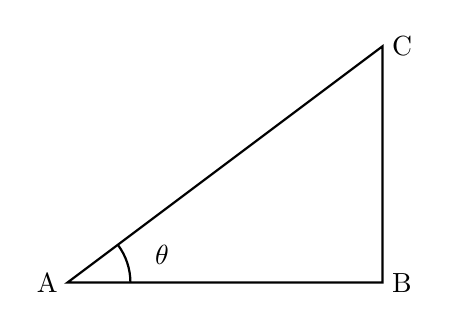
\begin{tikzpicture}[scale=1]

    % Define coordinates for the vertices of the right-angled triangle
    \coordinate (A) at (0, 0);
    \coordinate (B) at (4, 0);
    \coordinate (C) at (4, 3);

    % Draw the three sides of the triangle
    \draw[thick] (A) -- (B) -- (C) -- cycle;

    % Draw the arc for angle theta at vertex A
    % The arc starts from the horizontal line AB and sweeps up to the hypotenuse AC
    \draw[thick] (0.8, 0) arc (0:36.87:0.8);
    
    % Add the angle label theta inside the arc
    \node at (1.2, 0.35) {$\theta$};

    % Add labels to the vertices exactly where they appear
    \node[left] at (A) {A};
    \node[right] at (B) {B};
    \node[right] at (C) {C};

\end{tikzpicture}